\documentclass[11pt]{article}
\usepackage{amsmath}
\usepackage{amssymb}
\usepackage{graphicx}
\usepackage{tabularx}
\usepackage{fancyhdr}
\usepackage{lastpage}

% Page layout
\usepackage[top=1in, bottom=1in, left=1in, right=1in]{geometry}

% Header and footer
\pagestyle{fancy}
\fancyhf{}
\rfoot{Page \thepage}
\renewcommand{\headrulewidth}{0pt}

% Modified Question command with left-aligned number
\newcommand{\questiona}[2]{
    \noindent\textbf{Q#2.} #1 \hfill \textbf{[1 Mark]}
}

\newcommand{\questionb}[2]{
    \noindent\textbf{Q#2.} #1 \hfill \textbf{[2 Marks]}
}

\begin{document}

% Title section with horizontal line
\begin{center}
    \Large\textbf{GATE 2018 - Instrumentation Engineering (IN)} \\
    \large\textbf{General Aptitude and Technical Questions} \\
    \rule{\textwidth}{0.5pt} % Horizontal line below heading
\end{center}

\vspace{0.5cm}

% General Aptitude Section
\section*{General Aptitude}

\questiona{“When she fell down the \_\_\_\_\_, she received many \_\_\_\_\_ but little help.”}{1}
\begin{enumerate}
    \item[(A)] stairs, stares
    \item[(B)] stairs, stairs
    \item[(C)] stares, stairs
    \item[(D)] stares, stares
\end{enumerate}
\vspace{0.5cm}

\questiona{“In spite of being warned repeatedly, he failed to correct his \_\_\_\_\_\_ behaviour.”}{2}
\begin{enumerate}
    \item[(A)] rational
    \item[(B)] reasonable
    \item[(C)] errant
    \item[(D)] good
\end{enumerate}
\vspace{0.5cm}

\questiona{For \(0 \leq x \leq 2\pi\), \(\sin x\) and \(\cos x\) are both decreasing functions in the interval \_\_\_\_.}{3}
\begin{enumerate}
    \item[(A)] \((0, \frac{\pi}{2})\)
    \item[(B)] \((\frac{\pi}{2}, \pi)\)
    \item[(C)] \((\pi, \frac{3\pi}{2})\)
    \item[(D)] \((\frac{3\pi}{2}, 2\pi)\)
\end{enumerate}
\vspace{0.5cm}

\questiona{The area of an equilateral triangle is \(\sqrt{3}\). What is the perimeter of the triangle?}{4}
\begin{enumerate}
    \item[(A)] 2
    \item[(B)] 4
    \item[(C)] 6
    \item[(D)] 8
\end{enumerate}
\vspace{0.5cm}

\questiona{Arrange the following three-dimensional objects in the descending order of their volumes:
(i) A cuboid with dimensions 10 cm, 8 cm and 6 cm \\
(ii) A cube of side 8 cm \\
(iii) A cylinder with base radius 7 cm and height 7 cm \\
(iv) A sphere of radius 7 cm}{5}
\begin{enumerate}
    \item[(A)] (i), (ii), (iii), (iv)
    \item[(B)] (ii), (i), (iv), (iii)
    \item[(C)] (iii), (ii), (i), (iv)
    \item[(D)] (iv), (iii), (ii), (i)
\end{enumerate}
\vspace{0.5cm}

\questionb{An automobile travels from city A to city B and returns to city A by the same route. The speed of the vehicle during the onward and return journeys were constant at 60 km/h and 90 km/h, respectively. What is the average speed in km/h for the entire journey?}{6}
\begin{enumerate}
    \item[(A)] 72
    \item[(B)] 73
    \item[(C)] 74
    \item[(D)] 75
\end{enumerate}
\vspace{0.5cm}

\questionb{A set of 4 parallel lines intersect with another set of 5 parallel lines. How many parallelograms are formed?}{7}
\begin{enumerate}
    \item[(A)] 20
    \item[(B)] 48
    \item[(C)] 60
    \item[(D)] 72
\end{enumerate}
\vspace{0.5cm}

\questionb{To pass a test, a candidate needs to answer at least 2 out of 3 questions correctly. A total of 6,30,000 candidates appeared for the test. Question A was correctly answered by 3,30,000 candidates. Question B was answered correctly by 2,50,000 candidates. Question C was answered correctly by 2,60,000 candidates. Both questions A and B were answered correctly by 1,00,000 candidates. Both questions B and C were answered correctly by 90,000 candidates. Both questions A and C were answered correctly by 80,000 candidates. If the number of students answering all questions correctly is the same as the number answering none, how many candidates failed to clear the test?}{8}
\begin{enumerate}
    \item[(A)] 30,000
    \item[(B)] 2,70,000
    \item[(C)] 3,90,000
    \item[(D)] 4,20,000
\end{enumerate}
\vspace{0.5cm}

\questionb{If \(x^2 + x - 1 = 0\), what is the value of \(x^4 + \frac{1}{x^4}\)?}{9}
\begin{enumerate}
    \item[(A)] 1
    \item[(B)] 5
    \item[(C)] 7
    \item[(D)] 9
\end{enumerate}
\vspace{0.5cm}

\questionb{In a detailed study of annual crow births in India, it was found that there was relatively no growth during the period 2002 to 2004 and a sudden spike from 2004 to 2005. In another unrelated study, it was found that the revenue from cracker sales in India which remained fairly flat from 2002 to 2004, saw a sudden spike in 2005 before declining again in 2006. The solid line in the graph below refers to annual sale of crackers and the dashed line refers to the annual crow births in India. Choose the most appropriate inference from the above data.}{10}
\begin{center}
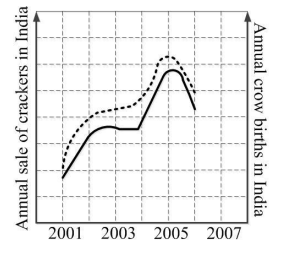
\includegraphics[width=0.5\textwidth]{figures/10.png}
\end{center}
\begin{enumerate}
    \item[(A)] There is a strong correlation between crow birth and cracker sales.
    \item[(B)] Cracker usage increases crow birth rate.
    \item[(C)] If cracker sale declines, crow birth will decline.
    \item[(D)] Increased birth rate of crows will cause an increase in the sale of crackers.
\end{enumerate}
\vspace{0.5cm}

\section*{Technical Section}

\questiona{Let \(N\) be a 3 by 3 matrix with real number entries. The matrix \(N\) is such that \(N^2 = 0\). The eigenvalues of \(N\) are}{1}
\begin{enumerate}
    \item[(A)] 0, 0, 0
    \item[(B)] 0, 0, 1
    \item[(C)] 0, 1, 1
    \item[(D)] 1, 1, 1
\end{enumerate}
\vspace{0.5cm}

\questiona{Let \(f_1(z) = z^2\) and \(f_2(z) = \bar{z}\) be two complex variable functions. Here \(\bar{z}\) is the complex conjugate of \(z\). Choose the correct answer.}{2}
\begin{enumerate}
    \item[(A)] Both \(f_1(z)\) and \(f_2(z)\) are analytic
    \item[(B)] Only \(f_1(z)\) is analytic
    \item[(C)] Only \(f_2(z)\) is analytic
    \item[(D)] Both \(f_1(z)\) and \(f_2(z)\) are not analytic
\end{enumerate}
\vspace{0.5cm}

\questiona{\(X\) and \(Y\) are two independent random variables with variances 1 and 2, respectively. Let \(Z = X - Y\). The variance of \(Z\) is}{3}
\begin{enumerate}
    \item[(A)] 0
    \item[(B)] 1
    \item[(C)] 2
    \item[(D)] 3
\end{enumerate}
\vspace{0.5cm}

\questiona{Consider two functions \(f(x) = (x - 2)^2\) and \(g(x) = 2x - 1\), where \(x\) is real. The smallest value of \(x\) for which \(f(x) = g(x)\) is \_\_\_\_\_.}{4}
\vspace{0.5cm}

\questiona{Consider a sequence of tossing of a fair coin where the outcomes of tosses are independent. The probability of getting the head for the third time in the fifth toss is}{5}
\begin{enumerate}
    \item[(A)] \(\frac{5}{16}\)
    \item[(B)] \(\frac{3}{16}\)
    \item[(C)] \(\frac{3}{5}\)
    \item[(D)] \(\frac{9}{16}\)
\end{enumerate}
\vspace{0.5cm}

\questiona{A series R-C circuit is excited by a \(1\angle 0^\circ\) V sinusoidal AC voltage source. The locus diagram of the phasor current \(I = (x + jy)\) A, when \(C\) is varied while keeping \(R\) fixed, is}{6}
\begin{center}
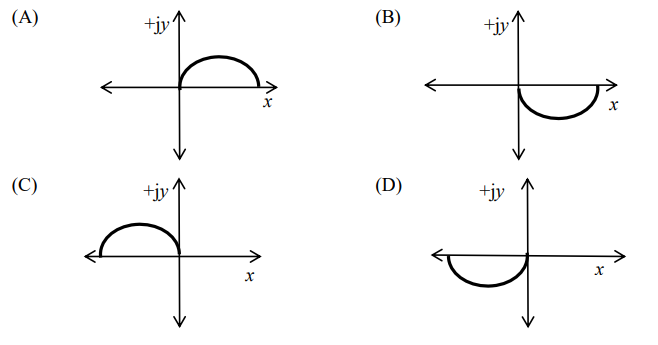
\includegraphics[width=0.8\textwidth]{figures/6.png}
\end{center}

\vspace{0.5cm}

\questiona{The Thevenin equivalent circuit representation across terminals p-q of the circuit shown in the figure is a}{7}
\begin{center}
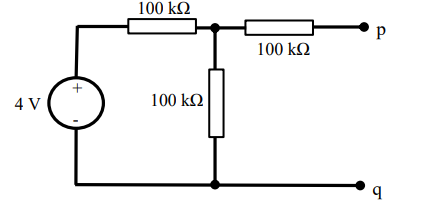
\includegraphics[width=0.5\textwidth]{figures/7.png}
\end{center}
\begin{enumerate}
    \item[(A)] 1 V source in series with 150 k\(\Omega\)
    \item[(B)] 1 V source in parallel with 100 k\(\Omega\)
    \item[(C)] 2 V source in series with 150 k\(\Omega\)
    \item[(D)] 2 V source in parallel with 200 k\(\Omega\)
\end{enumerate}
\vspace{0.5cm}

\questiona{A coil having an impedance of \((10 + j100)\ \Omega\) is connected in parallel to a variable capacitor as shown in figure. Keeping the excitation frequency unchanged, the value of the capacitor is changed so that parallel resonance occurs. The impedance across terminals p-q at resonance (in \(\Omega\)) is \_\_\_\_\_.}{8}
\begin{center}
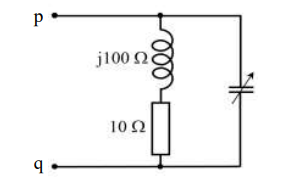
\includegraphics[width=0.5\textwidth]{figures/8.png}
\end{center}
\vspace{0.5cm}

\questiona{Two periodic signals \(x(t)\) and \(y(t)\) have the same fundamental period of 3 seconds. Consider the signal \(z(t) = x(-t) + y(2t + 1)\). The fundamental period of \(z(t)\) in seconds is}{9}
\begin{enumerate}
    \item[(A)] 1
    \item[(B)] 1.5
    \item[(C)] 2
    \item[(D)] 3
\end{enumerate}
\vspace{0.5cm}

\questiona{Consider signal \(x(t) = \begin{cases} 1, & |t| \leq 2 \\ 0, & |t| > 2 \end{cases}\). Let \(\delta(t)\) denote the unit impulse (Dirac-delta) function. The value of the integral \(\int_0^5 2x(t - 3)\delta(t - 4)dt\) is}{10}
\begin{enumerate}
    \item[(A)] 2
    \item[(B)] 1
    \item[(C)] 0
    \item[(D)] 3
\end{enumerate}
\vspace{0.5cm}

\questiona{An ideal square wave with period of 20 ms shown in the figure, is passed through an ideal low pass filter with cut-off frequency 120 Hz. Which of the following is an accurate description of the output?}{11}
\begin{center}
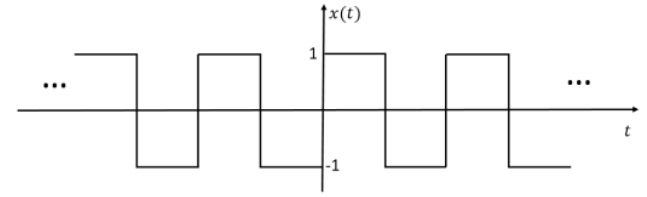
\includegraphics[width=0.5\textwidth]{figures/11.png}
\end{center}
\begin{enumerate}
    \item[(A)] Output is zero.
    \item[(B)] Output consists of both 50 Hz and 100 Hz frequency components.
    \item[(C)] Output is a pure sinusoid of frequency 50 Hz.
    \item[(D)] Output is a square wave of fundamental frequency 50 Hz.
\end{enumerate}
\vspace{0.5cm}

\questiona{An input \(p(t) = \sin(t)\) is applied to the system \(G(s) = \frac{s - 1}{s + 1}\). The corresponding steady state output is \(y(t) = \sin(t + \phi)\), where the phase \(\phi\) (in degrees), when restricted to \(0^\circ \leq \phi \leq 360^\circ\), is \_\_\_\_\_.}{12}
\vspace{0.5cm}

\questiona{The approximate phase response of \(\frac{100^2 e^{-0.01s}}{s^2 + 0.2s + 100^2}\) is}{13}
\begin{center}
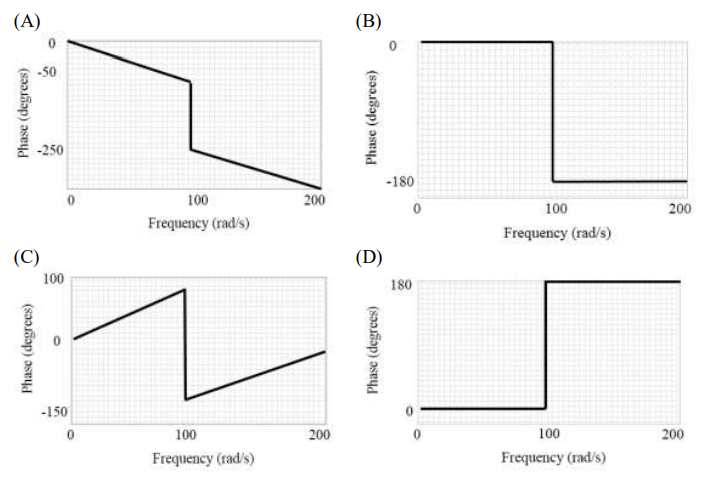
\includegraphics[width=0.8\textwidth]{figures/13.png}
\end{center}

\vspace{0.5cm}

\questiona{Consider the transfer function \(G(s) = \frac{2}{(s+1)(s+2)}\). The phase margin of \(G(s)\) in degrees is \_\_\_\_\_.}{14}
\vspace{0.5cm}

\questiona{In the given circuit, assume that the opamp is ideal and the transistor has a \(\beta\) of 20. The current \(I_o\) (in \(\mu A\)) flowing through the load \(Z_L\) is \_\_\_\_\_.}{15}
\begin{center}
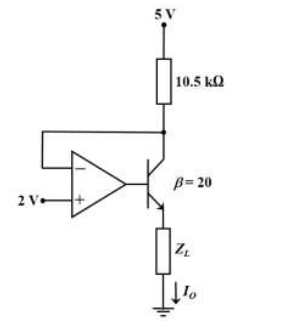
\includegraphics[width=0.5\textwidth]{figures/15.png}
\end{center}
\vspace{0.5cm}

\questiona{The diodes given in the circuit are ideal. At \(t = 60\ \text{ms}\), \(V_{pq}\) (in Volts) is \_\_\_\_\_.}{16}
\begin{center}
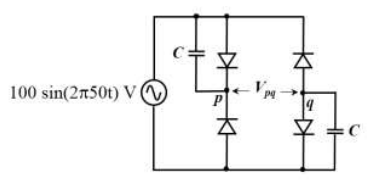
\includegraphics[width=0.5\textwidth]{figures/16.png}
\end{center}
\vspace{0.5cm}

\questiona{For the 3-bit binary counter shown in the figure, the output increments at every positive transition in the clock (CLK). Assume ideal diodes and the starting state of the counter as 000. If output high is 1 V and output low is 0 V, the current \(I\) (in mA) flowing through the 50 \(\Omega\) resistor during the 5th clock cycle is (up to one decimal place) \_\_\_\_\_.}{17}
\begin{center}
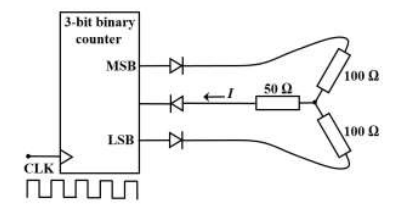
\includegraphics[width=0.5\textwidth]{figures/17.png}
\end{center}
\vspace{0.5cm}

\questiona{The representation of the decimal number \((27.625)_{10}\) in base-2 number system is}{18}
\begin{enumerate}
    \item[(A)] 11011.110
    \item[(B)] 11101.101
    \item[(C)] 11011.101
    \item[(D)] 10111.110
\end{enumerate}
\vspace{0.5cm}

\questiona{The number of comparators required for implementing an 8-bit flash analog-to-digital converter is}{19}
\begin{enumerate}
    \item[(A)] 8
    \item[(B)] 128
    \item[(C)] 255
    \item[(D)] 256
\end{enumerate}
\vspace{0.5cm}

\questiona{A voltage of \(6\cos(100\pi t)\) V is fed as y-input to a CRO. The waveform seen on the screen of the CRO is shown in the figure. The Y and X axes settings for the CRO are respectively}{20}
\begin{center}
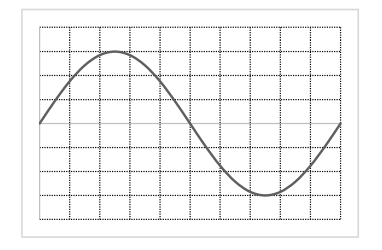
\includegraphics[width=0.5\textwidth]{figures/20.png}
\end{center}
\begin{enumerate}
    \item[(A)] 1 V/div and 1 ms/div
    \item[(B)] 1 V/div and 2 ms/div
    \item[(C)] 2 V/div and 1 ms/div
    \item[(D)] 2 V/div and 2 ms/div
\end{enumerate}
\vspace{0.5cm}

\questiona{A 300 V, 5 A, 0.2 pf low power factor wattmeter is used to measure the power consumed by a load. The wattmeter scale has 150 divisions and the pointer is on the 100th division. The power consumed by the load (in Watts) is \_\_\_\_\_.}{21}
\vspace{0.5cm}

\questiona{As shown in the figure, temperature \(\theta\) is measured using a K type thermocouple. It has a sensitivity of 40 \(\mu\)V/\(^\circ\)C. The gain (G) of the ideal instrumentation amplifier is 25. If the output \(V_o\) is 96 mV, then the value of \(\theta\) (in \(^\circ\)C) is \_\_\_\_\_.}{22}
\begin{center}
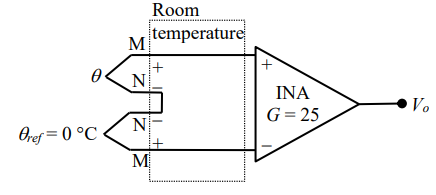
\includegraphics[width=0.5\textwidth]{figures/22.png}
\end{center}
\vspace{0.5cm}

\questiona{A piezoelectric pressure sensor has a bandpass characteristic with cut-off frequencies of 0.1 Hz and 1 MHz, and a sensitivity of 100 mV/kPa. The sensor is subjected to a static constant pressure of 100 kPa. Its steady-state output will be}{23}
\begin{enumerate}
    \item[(A)] 0 V
    \item[(B)] 0.1 V
    \item[(C)] 1 V
    \item[(D)] 10 V
\end{enumerate}
\vspace{0.5cm}

\questiona{An amplitude modulated signal is shown in the figure. The modulation index is (up to one decimal place) \_\_\_\_\_.}{24}
\begin{center}
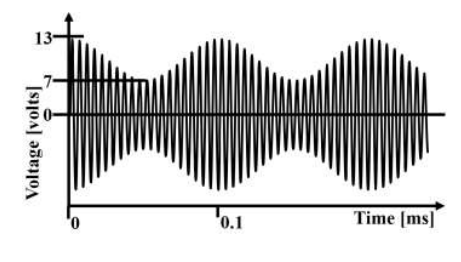
\includegraphics[width=0.5\textwidth]{figures/24.png}
\end{center}
\vspace{0.5cm}

\questiona{An optical pulse containing \(6 \times 10^6\) photons is incident on a photodiode and \(4.5 \times 10^6\) electron-hole pairs are created. The maximum possible quantum efficiency (in \%) of the photodiode is \_\_\_\_\_.}{25}
\vspace{0.5cm}

\questionb{Given \(\vec{F} = (x^2 - 2y)\hat{i} - 4yz\hat{j} + 4xz^2\hat{k}\), the value of the line integral \(\int_C \vec{F} \cdot d\vec{l}\) along the straight line \(C\) from (0,0,0) to (1,1,1) is}{26}
\begin{enumerate}
    \item[(A)] \(\frac{3}{16}\)
    \item[(B)] 0
    \item[(C)] \(-\frac{5}{12}\)
    \item[(D)] \(-1\)
\end{enumerate}
\vspace{0.5cm}

\questionb{Two bags A and B have equal number of balls. Bag A has 20\% red balls and 80\% green balls. Bag B has 30\% red balls, 60\% green balls and 10\% yellow balls. Contents of Bags A and B are mixed thoroughly and a ball is randomly picked from the mixture. What is the chance that the ball picked is red?}{27}
\begin{enumerate}
    \item[(A)] 20\%
    \item[(B)] 25\%
    \item[(C)] 30\%
    \item[(D)] 40\%
\end{enumerate}
\vspace{0.5cm}

\questionb{Consider the following system of linear equations:
\[
\begin{aligned}
3x + 2ky &= -2 \\
kx + 6y &= 2
\end{aligned}
\]
Here \(x\) and \(y\) are the unknowns and \(k\) is a real constant. The value of \(k\) for which there are infinite number of solutions is}{28}
\begin{enumerate}
    \item[(A)] 3
    \item[(B)] 1
    \item[(C)] \(-3\)
    \item[(D)] \(-6\)
\end{enumerate}
\vspace{0.5cm}

\questionb{Consider the following equations:
\[
\frac{\partial V(x, y)}{\partial x} = px^2 + y^2 + 2xy \\
\frac{\partial V(x, y)}{\partial y} = x^2 + qy^2 + 2xy
\]
where \(p\) and \(q\) are constants. \(V(x, y)\) that satisfies the above equations is}{29}
\begin{enumerate}
    \item[(A)] \(\frac{p x^3}{3} + \frac{q y^3}{3} + 2xy + 6\)
    \item[(B)] \(\frac{p x^3}{3} + \frac{q y^3}{3} + 5\)
    \item[(C)] \(\frac{p x^3}{3} + \frac{q y^3}{3} + x^2 y + x y^2 + xy\)
    \item[(D)] \(\frac{p x^3}{3} + \frac{q y^3}{3} + x^2 y + x y^2\)
\end{enumerate}
\vspace{0.5cm}

\questionb{In the given circuit, superposition is applied. When \(V_2\) is set to 0 V, the current \(I_2\) is -6 A. When \(V_1\) is set to 0 V, the current \(I_1\) is +6 A. Current \(I_3\) (in A) when both sources are applied will be (up to two decimal places) \_\_\_\_\_.}{30}
\begin{center}
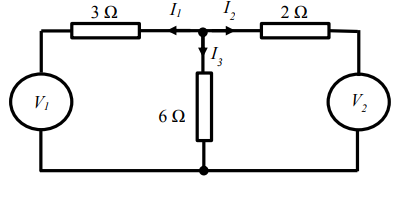
\includegraphics[width=0.5\textwidth]{figures/30.png}
\end{center}
\vspace{0.5cm}

\questionb{In the figure, an RLC load is supplied by a 230 V, 50 Hz single phase source. The magnitude of the reactive power (in VAr) supplied by the source is \_\_\_\_\_.}{31}
\begin{center}
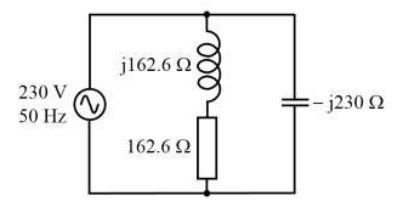
\includegraphics[width=0.5\textwidth]{figures/31.png}
\end{center}
\vspace{0.5cm}

\questionb{In the given circuit, the mesh currents \(I_1\), \(I_2\) and \(I_3\) are}{32}
\begin{center}
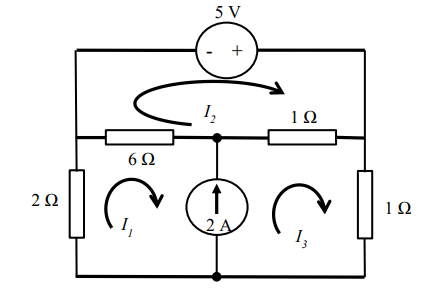
\includegraphics[width=0.5\textwidth]{figures/32.png}
\end{center}
\begin{enumerate}
    \item[(A)] \(I_1 = 1\) A, \(I_2 = 2\) A and \(I_3 = 3\) A
    \item[(B)] \(I_1 = 2\) A, \(I_2 = 3\) A and \(I_3 = 4\) A
    \item[(C)] \(I_1 = 3\) A, \(I_2 = 4\) A and \(I_3 = 5\) A
    \item[(D)] \(I_1 = 4\) A, \(I_2 = 5\) A and \(I_3 = 6\) A
\end{enumerate}
\vspace{0.5cm}

\questionb{The Fourier transform of a signal \(x(t)\), denoted by \(X(j\omega)\), is shown in the figure.
Let \(y(t) = x(t) + e^{jt}x(t)\). The value of Fourier transform of \(y(t)\) evaluated at the angular frequency \(\omega = 0.5\ \text{rad/s}\) is}{33}
\begin{center}
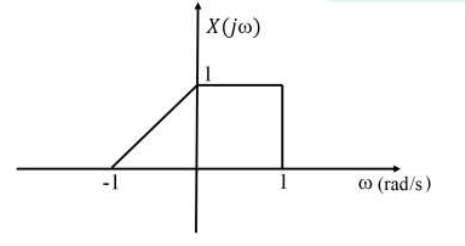
\includegraphics[width=0.5\textwidth]{figures/33.png}
\end{center}
\begin{enumerate}
    \item[(A)] 0.5
    \item[(B)] 1
    \item[(C)] 1.5
    \item[(D)] 2.5
\end{enumerate}
\vspace{0.5cm}

\questionb{Let \(y[n] = x[n] * h[n]\), where * denotes convolution and \(x[n]\) and \(h[n]\) are two discrete-time sequences. Given that the z-transform of \(y[n]\) is \(Y(z) = 2 + 3z^{-1} + z^{-2}\), the z-transform of \(p[n] = x[n] * h[n - 2]\) is}{34}
\begin{enumerate}
    \item[(A)] \(2 + 3z + z^{-2}\)
    \item[(B)] \(3z + z^{-2}\)
    \item[(C)] \(2z^2 + 3z + 1\)
    \item[(D)] \(2z^{-2} + 3z^{-3} + z^{-4}\)
\end{enumerate}
\vspace{0.5cm}

\questionb{For the sequence \(x[n] = \{1, -1, 1, -1\}\), with \(n = 0,1,2,3\), the DFT is computed as
\[
X(k) = \sum_{n=0}^{3} x[n] e^{-j \frac{2\pi}{4}nk}, \text{ for } k = 0,1,2,3.
\]
The value of \(k\) for which \(X(k)\) is not zero is}{35}
\begin{enumerate}
    \item[(A)] 0
    \item[(B)] 1
    \item[(C)] 2
    \item[(D)] 3
\end{enumerate}
\vspace{0.5cm}

\questionb{Consider the standard negative feedback configuration with \(G(s) = \frac{s^2 + 0.2s + 100}{s^2 - 0.2s + 100}\) and \(H(s) = \frac{1}{2}\). The number of clockwise encirclements of \((-1, 0)\) in the Nyquist plot of the loop transfer function \(G(s)H(s)\) is \_\_\_\_\_.}{36}
\vspace{0.5cm}

\questionb{Consider the linear system \(\dot{x} = \begin{bmatrix} -1 & 0 \\ 0 & -2 \end{bmatrix}x\), with initial condition \(x(0) = \begin{bmatrix} 1 \\ 1 \end{bmatrix}\). The solution \(x(t)\) for this system is}{37}
\begin{enumerate}
    \item[(A)] \(x(t) = \begin{bmatrix} e^{-t} & te^{-2t} \\ 0 & e^{-2t} \end{bmatrix} \begin{bmatrix} 1 \\ 1 \end{bmatrix}\)
    \item[(B)] \(x(t) = \begin{bmatrix} e^{-t} & 0 \\ 0 & e^{2t} \end{bmatrix} \begin{bmatrix} 1 \\ 1 \end{bmatrix}\)
    \item[(C)] \(x(t) = \begin{bmatrix} e^{-t} & -t^2 e^{-2t} \\ 0 & e^{-2t} \end{bmatrix} \begin{bmatrix} 1 \\ 1 \end{bmatrix}\)
    \item[(D)] \(x(t) = \begin{bmatrix} e^{-t} & 0 \\ 0 & e^{-2t} \end{bmatrix} \begin{bmatrix} 1 \\ 1 \end{bmatrix}\)
\end{enumerate}
\vspace{0.5cm}

\questionb{Consider a standard negative feedback configuration with \(G(s) = \frac{1}{(s+1)(s+2)}\) and \(H(s) = \frac{s + \alpha}{s}\). For the closed-loop system to have poles on the imaginary axis, the value of \(\alpha\) should be equal to (up to one decimal place) \_\_\_\_\_.}{38}
\vspace{0.5cm}

\questionb{Unit step response of a linear time invariant (LTI) system is given by \(y(t) = (1 - e^{-2t})u(t)\). Assuming zero initial condition, the transfer function of the system is}{39}
\begin{enumerate}
    \item[(A)] \(\frac{1}{s + 1}\)
    \item[(B)] \(\frac{2}{(s + 1)(s + 2)}\)
    \item[(C)] \(\frac{1}{s + 2}\)
    \item[(D)] \(\frac{2}{s + 2}\)
\end{enumerate}
\vspace{0.5cm}

\questionb{In the given relaxation oscillator, the opamps and the zener diodes are ideal. The frequency (in kHz) of the square wave output \(v_o\) is \_\_\_\_\_.}{40}
\begin{center}
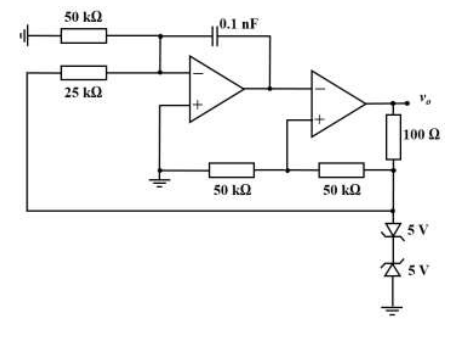
\includegraphics[width=0.5\textwidth]{figures/40.png}
\end{center}
\vspace{0.5cm}

\questionb{An opamp that is powered from a \(\pm5\) V supply is used to build a non-inverting amplifier having a gain of 15. The slew rate of the opamp is \(0.5 \times 10^6\ \text{V/s}\). For a sinusoidal input with amplitude of 0.3 V, the maximum frequency (in kHz) up to which it can be operated without any distortion is (up to one decimal place) \_\_\_\_\_.}{41}
\vspace{0.5cm}

\questionb{The circuit given uses ideal opamps. The current \(I\) (in \(\mu\)A) drawn from the source \(v_s\) is (up to two decimal places) \_\_\_\_\_.}{42}
\begin{center}
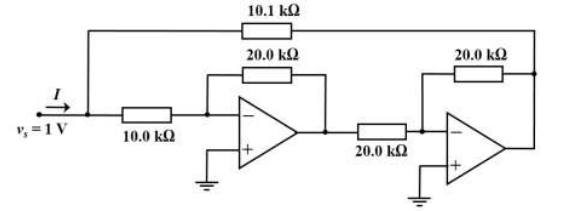
\includegraphics[width=0.5\textwidth]{figures/42.png}
\end{center}
\vspace{0.5cm}

\questionb{The product of sum expression of a Boolean function \(F(A, B, C)\) of three variables is given by
\[
F(A, B, C) = (A + B + \bar{C})(A + \bar{B} + \bar{C})(\bar{A} + B + C)(\bar{A} + \bar{B} + \bar{C})
\]
The canonical sum of product expression of \(F(A, B, C)\) is given by}{43}
\begin{enumerate}
    \item[(A)] \(\bar{A}\bar{B}C + \bar{A}BC + AB\bar{C} + ABC\)
    \item[(B)] \(\bar{A}\bar{B}\bar{C} + \bar{A}B\bar{C} + A\bar{B}C + AB\bar{C}\)
    \item[(C)] \(ABC + A\bar{B}\bar{C} + \bar{A}BC + \bar{A}\bar{B}\bar{C}\)
    \item[(D)] \(\bar{A}\bar{B}\bar{C} + \bar{A}BC + AB\bar{C} + ABC\)
\end{enumerate}
\vspace{0.5cm}

\questionb{A 2-bit synchronous counter using two J-K flip flops is shown. The expressions for the inputs to the J-K flip flops are also shown in the figure. The output sequence of the counter starting from \(Q_1Q_2 = 00\) is}{44}
\begin{center}
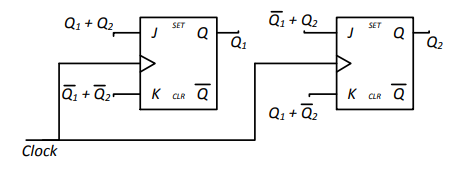
\includegraphics[width=0.5\textwidth]{figures/44.png}
\end{center}
\begin{enumerate}
    \item[(A)] 00 \(\rightarrow\) 11 \(\rightarrow\) 10 \(\rightarrow\) 01 \(\rightarrow\) 00 ...
    \item[(B)] 00 \(\rightarrow\) 01 \(\rightarrow\) 10 \(\rightarrow\) 11 \(\rightarrow\) 00 ...
    \item[(C)] 00 \(\rightarrow\) 01 \(\rightarrow\) 11 \(\rightarrow\) 10 \(\rightarrow\) 00 ...
    \item[(D)] 00 \(\rightarrow\) 10 \(\rightarrow\) 11 \(\rightarrow\) 01 \(\rightarrow\) 00 ...
\end{enumerate}
\vspace{0.5cm}

\questionb{A portion of an assembly language program written for an 8-bit microprocessor is given below along with explanations. The code is intended to introduce a software time delay. The processor is driven by a 5 MHz clock. The time delay (in \(\mu\)s) introduced by the program is \_\_\_\_\_.}{45}
\begin{center}
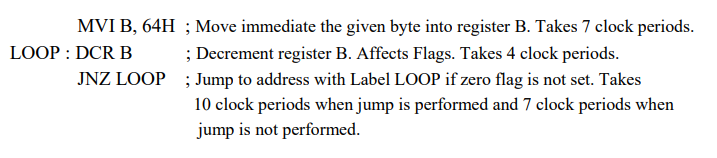
\includegraphics[width=0.8\textwidth]{figures/45.png}
\end{center}
\vspace{0.5cm}

\questionb{The Boolean function \(F(X, Y)\) realized by the given circuit is}{46}
\begin{center}
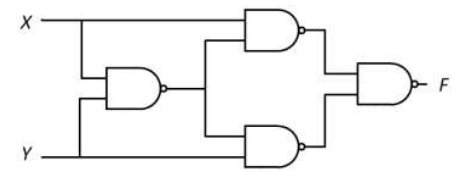
\includegraphics[width=0.5\textwidth]{figures/46.png}
\end{center}
\begin{enumerate}
    \item[(A)] \(\bar{X}Y + X\bar{Y}\)
    \item[(B)] \(\bar{X}\bar{Y} + XY\)
    \item[(C)] \(X + Y\)
    \item[(D)] \(\bar{X} \cdot \bar{Y}\)
\end{enumerate}
\vspace{0.5cm}

\questionb{The voltage and current drawn by a resistive load are measured with a 300 V voltmeter of accuracy \(\pm1\%\) of full scale and a 5 A ammeter of accuracy \(\pm0.5\%\) of full scale. The readings obtained are 200 V and 2.5 A. The limiting error (in \%) in computing the load resistance is (up to two decimal places) \_\_\_\_\_.}{47}
\vspace{0.5cm}

\questionb{A high Q coil having distributed (self) capacitance is tested with a Q-meter. First resonance at \(\omega_1 = 10^6\) rad/s is obtained with a capacitance of 990 pF. The second resonance at \(\omega_2 = 2 \times 10^6\) rad/s is obtained with a 240 pF capacitance. The value of the inductance (in mH) of the coil is (up to one decimal place) \_\_\_\_\_.}{48}
\vspace{0.5cm}

\questionb{The inductance of a coil is measured using the bridge shown in the figure. Balance (D = 0) is obtained with \(C_1 = 1\) nF, \(R_1 = 2.2\) M\(\Omega\), \(R_2 = 22.2\) k\(\Omega\), \(R_4 = 10\) k\(\Omega\). The value of the inductance \(L_x\) (in mH) is \_\_\_\_\_.}{49}
\begin{center}
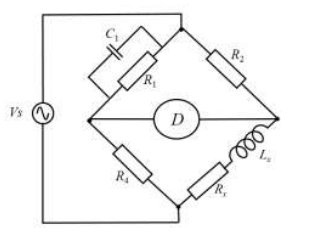
\includegraphics[width=0.5\textwidth]{figures/49.png}
\end{center}
\vspace{0.5cm}

\questionb{The average velocity \(v\) of flow of clear water in a 100 cm (inner) diameter tube is measured using the ultrasonic flow meter as shown in the figure. The angle \(\theta\) is \(45^\circ\). The measured transit times are \(t_1 = 0.9950\) ms and \(t_2 = 1.0000\) ms. The velocity \(v\) (in m/s) in the pipe is (up to one decimal place) \_\_\_\_\_.}{50}
\begin{center}
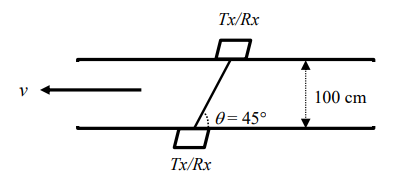
\includegraphics[width=0.5\textwidth]{figures/50.png}
\end{center}
\vspace{0.5cm}

\questionb{A 1000 \(\Omega\) strain gauge (\(R_g\)) has a gauge factor of 2.5. It is connected in the bridge as shown in the figure. The strain gauge is subjected with a positive strain of 400 \(\mu\)m/m. The output \(V_o\) (in mV) of the bridge is (up to two decimal places) \_\_\_\_\_.}{51}
\begin{center}
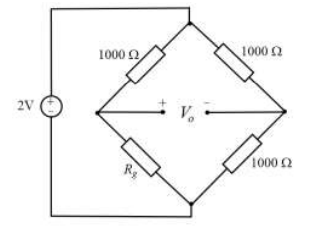
\includegraphics[width=0.5\textwidth]{figures/51.png}
\end{center}
\vspace{0.5cm}

\questionb{Assuming ideal opamp, the RMS voltage (in mV) in the output \(V_o\) only due to the 230 V, 50 Hz interference is (up to one decimal place) \_\_\_\_\_.}{52}
\begin{center}
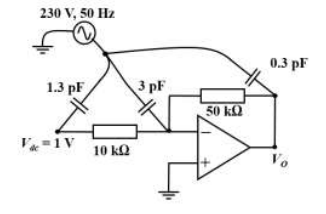
\includegraphics[width=0.5\textwidth]{figures/52.png}
\end{center}
\vspace{0.5cm}

\questionb{The sampling rate for Compact Discs (CDs) is 44,000 samples/s. If the samples are quantized to 256 levels and binary coded, the corresponding bit rate (in bits per second) is \_\_\_\_\_.}{53}
\vspace{0.5cm}

\questionb{A Michelson Interferometer using a laser source of wavelength \(\lambda_0 = 500\) nm, with both the mirrors (\(M_1\) \& \(M_2\)) fixed and positioned equidistant from the splitter/combiner is shown in the figure. When a dielectric plate of refractive index \(n = 1.5\), of thickness \(t\), is placed in front of the mirror \(M_2\), a dark fringe is observed on the detector. When the dielectric plate is removed without changing the position of the mirrors, a bright fringe is observed on the detector. The minimum thickness \(t\) (in nm) of the dielectric is \_\_\_\_\_.}{54}
\begin{center}
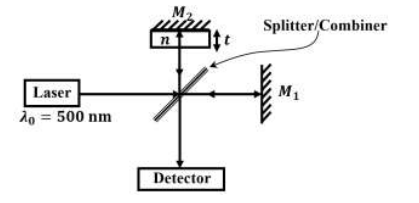
\includegraphics[width=0.5\textwidth]{figures/54.png}
\end{center}
\vspace{0.5cm}

\questionb{A multi-mode optical fiber with a large core diameter has a core refractive index \(n_1 = 1.5\) and cladding refractive index \(n_2 = 1.4142\). The maximum value of \(\theta_A\) (in degrees) for which the incident light from air will be guided in the optical fiber is \(\pm\) \_\_\_\_\_.}{55}
\vspace{5cm}

\begin{center}
\textbf{END OF THE QUESTION PAPER} \\
\rule{\textwidth}{0.5pt}
\end{center}

\end{document}
